\section{Mobility}

\begin{frame}
	\frametitle{Outline}
	\begin{tcolorbox}[coltitle=yellow!50!black,colframe=magenta!25,split=.2,title=Freedom and Structure]
		Freedoms, Constraints, and Mobility.
		\tcblower
		Motion of linkages: Screws, and spatial motions.
		\vspace{.2cm}
		\newline
		Freedom and Mobility: Freedoms, unfreedoms, connectivity, mobility;
		\vspace{.2cm}
		\newline
		Gr{\"u}bler-Kutzbach's mobility criterion and examples.
	\end{tcolorbox}
\end{frame}
 


\begin{frame}
	\frametitle{Degrees of Freedom and Structure}
	%		
	\begin{definition}[Connection Degree]
		For any  \textcolor{blue}{manipulator joint}, we shall mean its \textcolor{red}{connection degree} to be the \textcolor{red}{number of links attached it}.
	\end{definition}
	%	
	\begin{block}{Quiz}
		What is the connection degree of the u-joints of a Stewart-Gough platform.
	\end{block}
\end{frame}

	\begin{frame}
	\frametitle{Members and Dual Graphs}			
	%
	\begin{tcolorbox}[colframe=blue!80!green, title=Dual graph of a Stewart platform, coltitle=white!80,toggle enlargement=none]
		\begin{columns}[b]
			\begin{column}{\linewidth}			
				\begin{figure}
					\centering 
					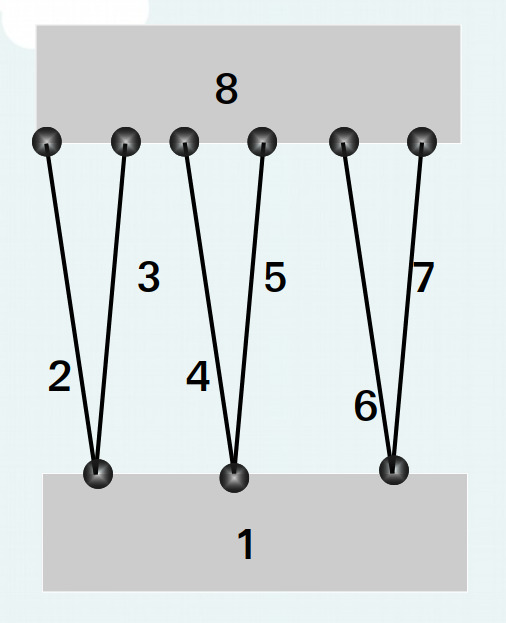
\includegraphics[width=.5\textwidth]{figures/dualgraph_stewart.jpg}
				\end{figure}
			\end{column}	
		\end{columns}
	\end{tcolorbox}
\label{fig:dualgraph}
\end{frame}

\begin{frame}
	\frametitle{Degrees of Freedom and Structure}
	%
	\begin{block}{Members and Freedoms}
		\textcolor{blue}{Degrees of freedoms (or freedoms)} concerns the \textcolor{red}{relative motion of members of a pair} that do not touch one another directly. 
	\end{block}
	%
	\begin{block}{Connectivity}
		By the dual graph of the Stewart platform as seen on Frame \autoref{fig:dualgraph}, the total number of freedoms that \textcolor{red}{connect the two members} (1 and 8) that do not connect to one another directly is \textcolor{blue}{six}. 
	\end{block}
\end{frame}


\begin{frame}
	\frametitle{Planar Linkages}	
	\begin{block}{Four Bar Linkages}
		\begin{columns}[b]
			\begin{column}{\linewidth}		
				\centering 
				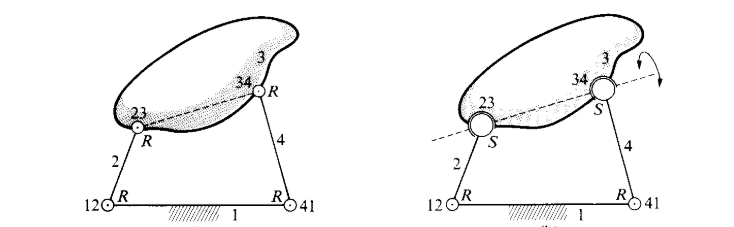
\includegraphics[width=\textwidth]{../Notes/figures/four-bar-linkage.png}
			\end{column}	
		\end{columns}
		\note{The planar $RRRR$ linkage, (\textit{left}) is modified in (\textit{right}) to an $RSSR$ linkage to allow spatial spin-movement of the coupler 3; the connectivity $\mathscr{C}_{13}=2$.}
		\footnotesize{Reprinted from Hunt, 1977: Kinematic Geometry of Mechanisms.}
	\end{block}
	\label{fig:4bar_hunt}
\end{frame}

\begin{frame}
	\frametitle{Freedom from Connectivity}			
	%
	\begin{tcolorbox}[colframe=blue!80!green, title=A (Hacked) Four-Bar Linkage, coltitle=white!80,toggle enlargement=none]
		\begin{columns}[b]
			\begin{column}{.45\linewidth}			
				\begin{figure}
					\centering 
					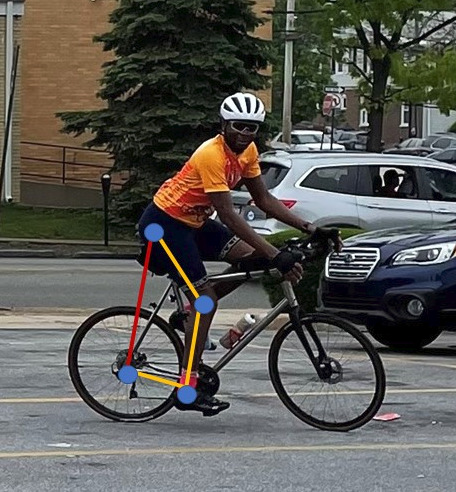
\includegraphics[width=\textwidth]{figures/4bar_me.jpg}
				\end{figure}
			\end{column}
		\begin{column}{.45\linewidth}			
			\begin{figure}
			\centering 
			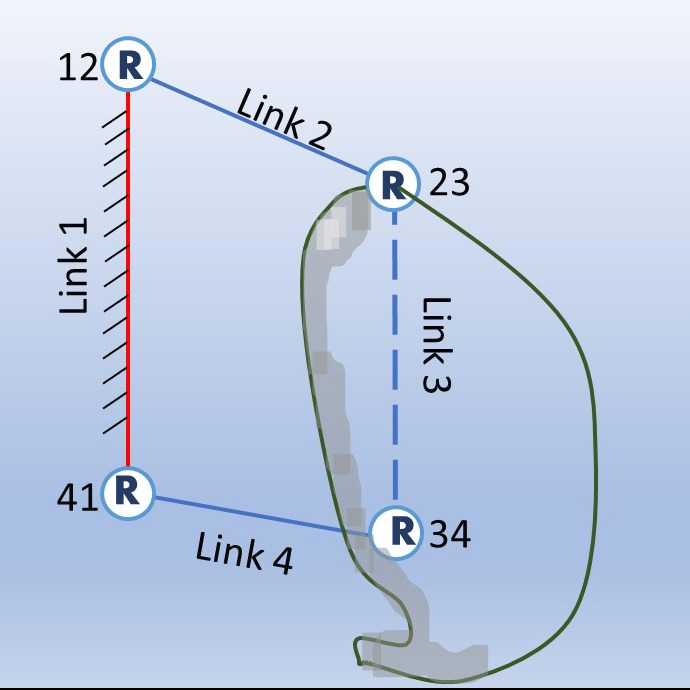
\includegraphics[width=\textwidth]{figures/4bardual.jpg}
			\end{figure}
		\end{column}	
		\end{columns}
	\end{tcolorbox}
	\label{fig:4bar}
\end{frame}


\begin{frame}
	\frametitle{The Four Bar Linkage}
	%
	\begin{block}{Couplings and Freedom}
		
		Links $2 \& 4$ complete a \textcolor{cyan}{coupling or connection} between links $1 \& 3$. 
	\end{block}
	%
	\begin{block}{Connectivity}
		The $R$-pairs are said to have a \textcolor{magenta}{connectivity} of  $\mathscr{C}_{ij}=1$ for all $i,j=1,2,3,4$. Thus, total degree of freedom is $1$.
	\end{block}
\end{frame}

\begin{frame}
	\frametitle{Mobility of Mechanisms}
	%
	\begin{block}{The Mobility and Relative Mobility, $\mathfrak{M}$}
		Simply put, the number of a mechanism's freedoms is its \textcolor{cyan}{mobility}, or \textcolor{cyan}{relative mobility},  $\mathfrak{M}$.  
	\end{block}
	%
	\begin{block}{The Mobility, $\mathfrak{M}$}
		It specifies the \textcolor{green}{independent variables} needed to \textcolor{pink}{determine every relative location} of a \textcolor{red}{mechanism's members}  with respect to one another.
	\end{block}
	%
	\begin{block}{A Note on Serial and Parallel Mobility}
		A little tricky to determine for parallel mechanisms but straightforward for serial mechanisms.
	\end{block}
\end{frame}

\begin{frame}
	\frametitle{Mobility of Mechanisms}
	%
	\begin{block}{Quiz}
		What is the mobility $\mathfrak{M}$ of the $RSSR$ four bar linkage of Frame \ref{fig:4bar_hunt}? Why?
	\end{block}
	%
	\begin{block}{Quiz}
		What is the mobility $\mathfrak{M}$ of the $RRRR$ four bar linkage of Frame \ref{fig:4bar}? Why?
	\end{block}
	%
	\begin{definition}[The mobility criterion (well, not yet)]
		Let's not get ahead of ourselves. A little introduction to screws are in order for us to grasp the \textcolor{red}{Gr{\"u}bler-Kutzbach} mobility criterion.
	\end{definition}
\end{frame}


\subsection{Screws}
\begin{frame}
	\frametitle{Unique Location of a Rigid Body in 3D Space}
	%
	\begin{tcolorbox}[top=0mm, title=Inhomogeneity of Displacements and Angles]
		Quiz: Three translations and three rotations are ill-posed for uniquely determining the freedoms of a body. Why?
		\tcblower
		They are \textcolor{green}{not homogeneous}. 
		\begin{description}
			\item For true \textcolor{blue}{kinematic wholeness and generality}, displacement that is \textcolor{red}{purely translatory} and \textcolor{red}{purely rotary} is needed.
		\end{description}
	\end{tcolorbox}
\end{frame}

\begin{frame}
	\frametitle{Screws for Kinematic Generality}
	%
	\begin{block}{Need for Screws}
		From a kinematic standpoint, \textcolor{red}{six homogeneous screw coordinates} -- each having an \textcolor{cyan}{independent screw freedom} -- are needed to \textcolor{red}{uniquely determine a rigid body's location}.
	\end{block}
	%
	\begin{columns}[b]
		\begin{column}{.7\columnwidth}
			\begin{definition}[What is a screw anyway?]
				A \textcolor{blue}{screw} is a \textcolor{red}{straight line} in space, called \textcolor{blue}{the axis}, with an associated direction, called \textcolor{blue}{pitch}, $p$.
			\end{definition}
		\end{column}
		\begin{column}{.25\columnwidth}
			\centering
			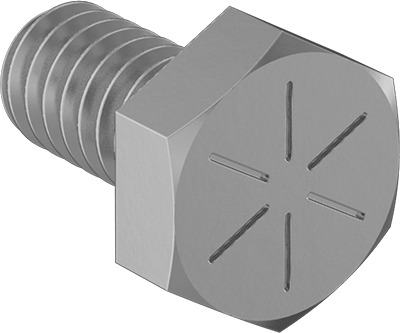
\includegraphics[width=\textwidth]{figures/screw.jpg}
		\end{column}
	\end{columns}
\end{frame}

\begin{frame}
	\frametitle{Unique Location of a Rigid Body in 3D Space}
	%
	\begin{columns}[b]
		\begin{column}{.65\columnwidth}
			\begin{definition}[Screw Coordinates]
				Six-vector, $\bm{s}$, related to the Pl{\"u}cker coordinates (see right inset) parameterize a screw i.e. $\bm{s}=\left(s_1, s_2, s_3, s_4, s_5, s_6\right)$.
			\end{definition}
		\end{column}
		\begin{column}{.3\columnwidth}
			\centering
			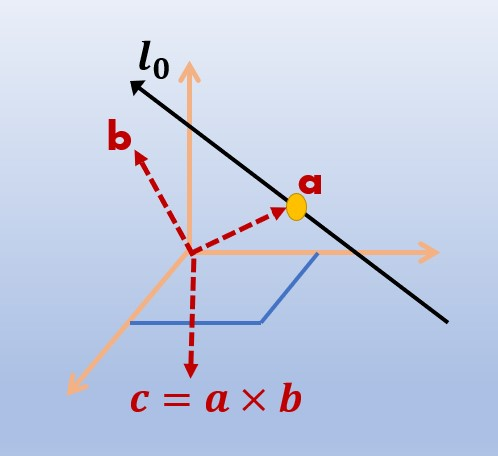
\includegraphics[width=\textwidth]{figures/plucker_coords.jpg}
		\end{column}
		\label{fig:plucker}
	\end{columns}
	%
	\begin{block}{Pl{\"u}cker Coordinates}
		Let \textcolor{red}{$\bm{a}$} be a point on line $\bm{\ell}_0$. Let \textcolor{red}{$\bm{a}$}'s direction cosine vector (to be introduced shortly) be \textcolor{red}{$\bm{b}$}. Then, its binormal (moment) vector is \textcolor{red}{$\bm{c=a\times b}$}. We say the pair \textcolor{red}{$(\bm{b},\bm{c})$} is the \textcolor{blue}{Pl{\"u}cker Coordinates} of the point  \textcolor{red}{$\bm{a}$ on axis $\bm{\ell}_0$}.
	\end{block}
\end{frame}


\subsection{Pl{\"u}cker coordinates}
\begin{frame}
	\frametitle{Screws and Pl{\"u}cker Coordinates Relationship}
	%
	\begin{block}{Screw axis and Pl{\"u}cker Coordinates Relationship}
		\begin{align}
			b_1 &= s_1, \quad b_2 = s_2, \quad b_3 = s_3 \\
			c_1 &= s_4 - ps_1, \quad c_2 = s_5-ps_2, \quad c_3 = s_6 - ps_3.
		\end{align}
	$p$: pitch! How to find it?
	\end{block}
	%
	\begin{block}{Screw and Pl{\"u}cker Coordinates Relationship}
		Suppose that 
		\begin{align}
			h &= \sqrt{b_1^2+b_2^2+b_3^2}.
		\end{align}
		Then $(\bm{b}/h, \bm{c}/h)$ are respectively the direction cosines of the line, $l_0$ and its moment.
	\end{block}
\end{frame}

\begin{frame}
	\frametitle{Pitch and Magnitude of the screw}	
	\begin{block}{Pitch of a screw}
		\begin{align}
			p &= \dfrac{s_1 \, s_4 + s_2 \, s_5 + s_3 \, s_6}{\sqrt{s_1^2 + s_2^2 + s_3^2}}, \\
			\mid s \mid &= \sqrt{s_1^2 + s_2^2 + s_3^2} \quad \text{if } p \neq \infty \\
			\mid s \mid &= \sqrt{s_4^2 + s_5^2 + s_6^2} \quad \text{if } p = \infty
		\end{align}
	\end{block}
\end{frame}
%
\begin{frame}
	\frametitle{Pl{\"u}cker Coordinates Example}
	\begin{block}{Chasles' Theorem Applied to The Serret-Frenet Frame}
		Consider a spatial curve $\bm{C}$ on the elephant continuum trunk shown earlier. Suppose $\bm{C}$ is parameterized by its arc length $\bm{s} \in [0, 1]$. For a point $\bm{x}=\left[x, y, z\right]^T$ on $\bm{C}$, the unit tangent vector to $\bm{C}$ is $\bm{t}=\bm{dx}/\bm{ds}$. Denote by $\bm{n}$ the principal normal to $\bm{C}$ at $\bm{n}$; then we must have $\bm{b}=\bm{t}\times \bm{n}$ as the binormal. We say $(\bm{b},\bm{n})$ together form the Pl{\"u}cker coordinates of the tangent $\bm{t}$.
	\end{block}
	%
	%
	\begin{columns}[]
		\begin{column}{.5\columnwidth}
			\centering
			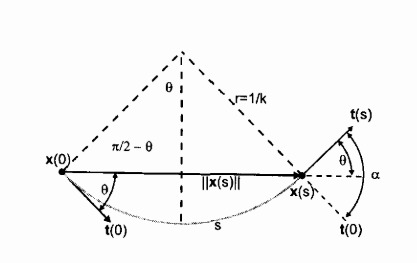
\includegraphics[width=\textwidth]{figures/serret.jpg}
		\end{column}
	\end{columns}
\end{frame}

\begin{frame}
	\frametitle{Pl{\"u}cker Coordinates Example}
	%
	\begin{block}{Poinsot's Theorem Quiz on a  Force and its Moment}
		Suppose that a force $\bm{F}$  acts at the point $\bm{a}$ in the image of Frame \ref{fig:plucker}. What are the Pl{\"u}cker coordinates of the \textcolor{red}{line of force}?
	\end{block}
	%
	\begin{block}{ Homogeneous Coordinates!}
		\textcolor{blue}{Pl{\"u}cker Coordinates} give six unit parameters of a point on a line. Pl{\"u}cker Coordinates are in \textcolor{red}{homogeneous coordinates}!
	\end{block}
\end{frame}

\note{
\begin{frame}
	%
	\begin{block}{Poinsot's Theorem Quiz on a  Force and its Moment}
		Imagine that a force $\bm{F}$ is acting at the point $\bm{a}$ in the image of Frame \ref{fig:plucker}. Suppose that $\bm{\tau}$ is torque acting along the normal to point $\bm{a}$.  Then $(\bm{f,\tau})$ are the Pl{\"u}cker  coordinates of the \textcolor{red}{line of force}.
	\end{block}
	%
	\begin{block}{Arithmetics on Screws}
		Scalar and vector arithmetic operations are valid on infinitesimal  screws e.g.
		\begin{align}
			c_1 \bm{s}_1 + c_2 \bm{s}_2 = 0 \text{ for } c_1, \, c_2 \neq 0 \text{ on screws } \bm{s}_1, \bm{s}_2.
		\end{align}
	\end{block}
\end{frame}
}

\subsection{Freedoms and Constraints}
\begin{frame}
	\frametitle{Freedoms, Unfreedoms, and Mobility}
	%
	\begin{block}{Freedom and Constraints}
		Suppose a screw $\bm{f}=(f_1,\cdots, f_6)$ ``fixes" a body in 3D space. 
		\begin{description}
			\item Each \textcolor{red}{constraint} $u_i \neq f_j$ for $(i,j)\in \{1,\cdots,6\}$.
			%
			\item Rather each \textcolor{red}{$u_i$} has influence on every $\{f_i\}_{i=1}^{6}$.
			%
			\item Each $u_i$ from the six independent equations, $g(s_1, s_2, s_3, s_4, s_5, s_6)=0$, suppresses a \textcolor{cyan}{freedom}, $f_i$.
			%
			\item Progressively relaxing each \textcolor{red}{$u_i$}, \textcolor{red}{or unfreedom}, adds an extra body $f_i$.
		\end{description}
	\end{block}
	%
\end{frame}


\begin{frame}
	\frametitle{Freedoms, Unfreedoms, and Mobility}
	%
	\begin{block}{Freedom and Unfreedoms}
		Suppose the total \textcolor{blue}{freedoms} is $\bm{f}$ and the total \textcolor{red}{unfreedoms} is $\bm{u}$, then
		\begin{description}
			\item $\bm{u}+\bm{f}=6.$
			\label{eq:freedomunfreedom}
		\end{description}
	Note: A rigid body's freedoms is also referred to the dimension of  its \textcolor{blue}{configuration space}.
	\end{block}
	%
	\begin{block}{Relative Freedoms}
		Suppose there are a total of $n$ \textcolor{red}{unconstrained} bodies. Suppose further that we choose one out of the bodies as a reference body. Then the total number of \textcolor{green}{relative freedoms} is $6(n-1)$.
	\end{block}
\end{frame}

\begin{frame}
	\frametitle{Freedoms, Unfreedoms, and Mobility}
	\begin{block}{Constraints and Joints}
		Now, consider $k$ \textcolor{red}{independent constraints}\footnote{NB: The total \textit{allowable} constraints is 5 for a body in relative motion. It is 6 for a fully rigid body.} such as \textcolor{blue}{joints} \textcolor{green}{along points, lines, curves or surfaces}.
	\end{block}
	
	\begin{block}{The Mobility Criterion}
		Let the \textcolor{red}{constraint} of joint, $i$ (e.g. a joint along points, lines, curves or surfaces) be $u_i$. Then the mobility criterion $\mathfrak{M}$ is
		\begin{align}
			\mathfrak{M}=6(n-1) - \sum_{i=1}^{k}u_i.
		\end{align}
	\end{block}
\end{frame}

\subsection{Mobility Criterion}
\begin{frame}
	\frametitle{ General Gr{\"u}bler-Kutzbach Mobility Criterion}	
	\begin{block}{ General Gr{\"u}bler-Kutzbach Mobility Criterion}
		Recall that $\sum_i u_i + f_i = 6$ from Frame \eqref{eq:freedomunfreedom} so that 
		\begin{align}
			\mathfrak{M}=6(n-k-1) - \sum_{i=1}^{f}f_i.
			\label{grubler}
		\end{align}
	\end{block}
	
	\begin{block}{Exceptions: Relative Planar and Spherical Motions}
		For bodies restricted to relative planar or spherical  motions, the total freedoms + constraints is 3 (not 6)! %Therefore, 
		\begin{align}
			\mathfrak{M}=3(n-k-1) - \sum_{i=1}^{f}f_i.
			\label{grubler}
		\end{align}
	\end{block}
\end{frame}

\begin{frame}
	\frametitle{ General Gr{\"u}bler-Kutzbach Criterion References}
		
	\begin{block}{The Gr{\"u}bler-Kutzbach Mobility Criterion References}
		Attributed to Gr{\"u}bler: 
		\begin{description}
			\item \footnotesize{Schoenflies, Arthur, and M. Grübler. ``Kinematik." In Encyklopädie der Mathematischen Wissenschaften mit Einschluss ihrer Anwendungen, pp. 190-278. Vieweg+Teubner Verlag, Wiesbaden, 1908};
			\item \footnotesize{Grübler, Martin Fürchtegott. Getriebelehre: eine Theorie des Zwanglaufes und der ebenen Mechanismen. Springer, 1917}.
		\end{description}
	and Kutzbach:
		\begin{description}
			\item \footnotesize{Kutzbach, Karl. "Mechanische leitungsverzweigung, ihre gesetze und anwendungen." Maschinenbau 8, no. 21 (1929): 710-716.}
		\end{description}
	\end{block}
\end{frame}

\begin{frame}
	\frametitle{Loops}	
	\begin{block}{Loops}
		A \textcolor{blue}{kinematic chain} often comprises \textcolor{blue}{members} called \textcolor{green}{loops}. 
	\end{block}
	
	\begin{block}{Binary Link}
		Members in a \textcolor{blue}{binary link} constitute a \textcolor{green}{single loop}. Example: The four-bar linkage. 
	\end{block}	
	
	\begin{block}{Single loops}
		For \textcolor{blue}{single loops}, $k=n$ so that $\mathfrak{M}=\sum_{i=1}^{f} f_i - 6$. 
	\end{block}
	
	\begin{block}{Mobility of Mechanisms}
		$\mathfrak{M}\le 1$ for at least one actuator-pair to produce mobility at a successor joint which depends on that actuator-pair's input. 
	\end{block}
\end{frame}


%
\begin{frame}
	\frametitle{Mobility of Common Robot Configurations}
	%
	\begin{columns}[]
		%
		\begin{column}{.5\linewidth}
			\centering
			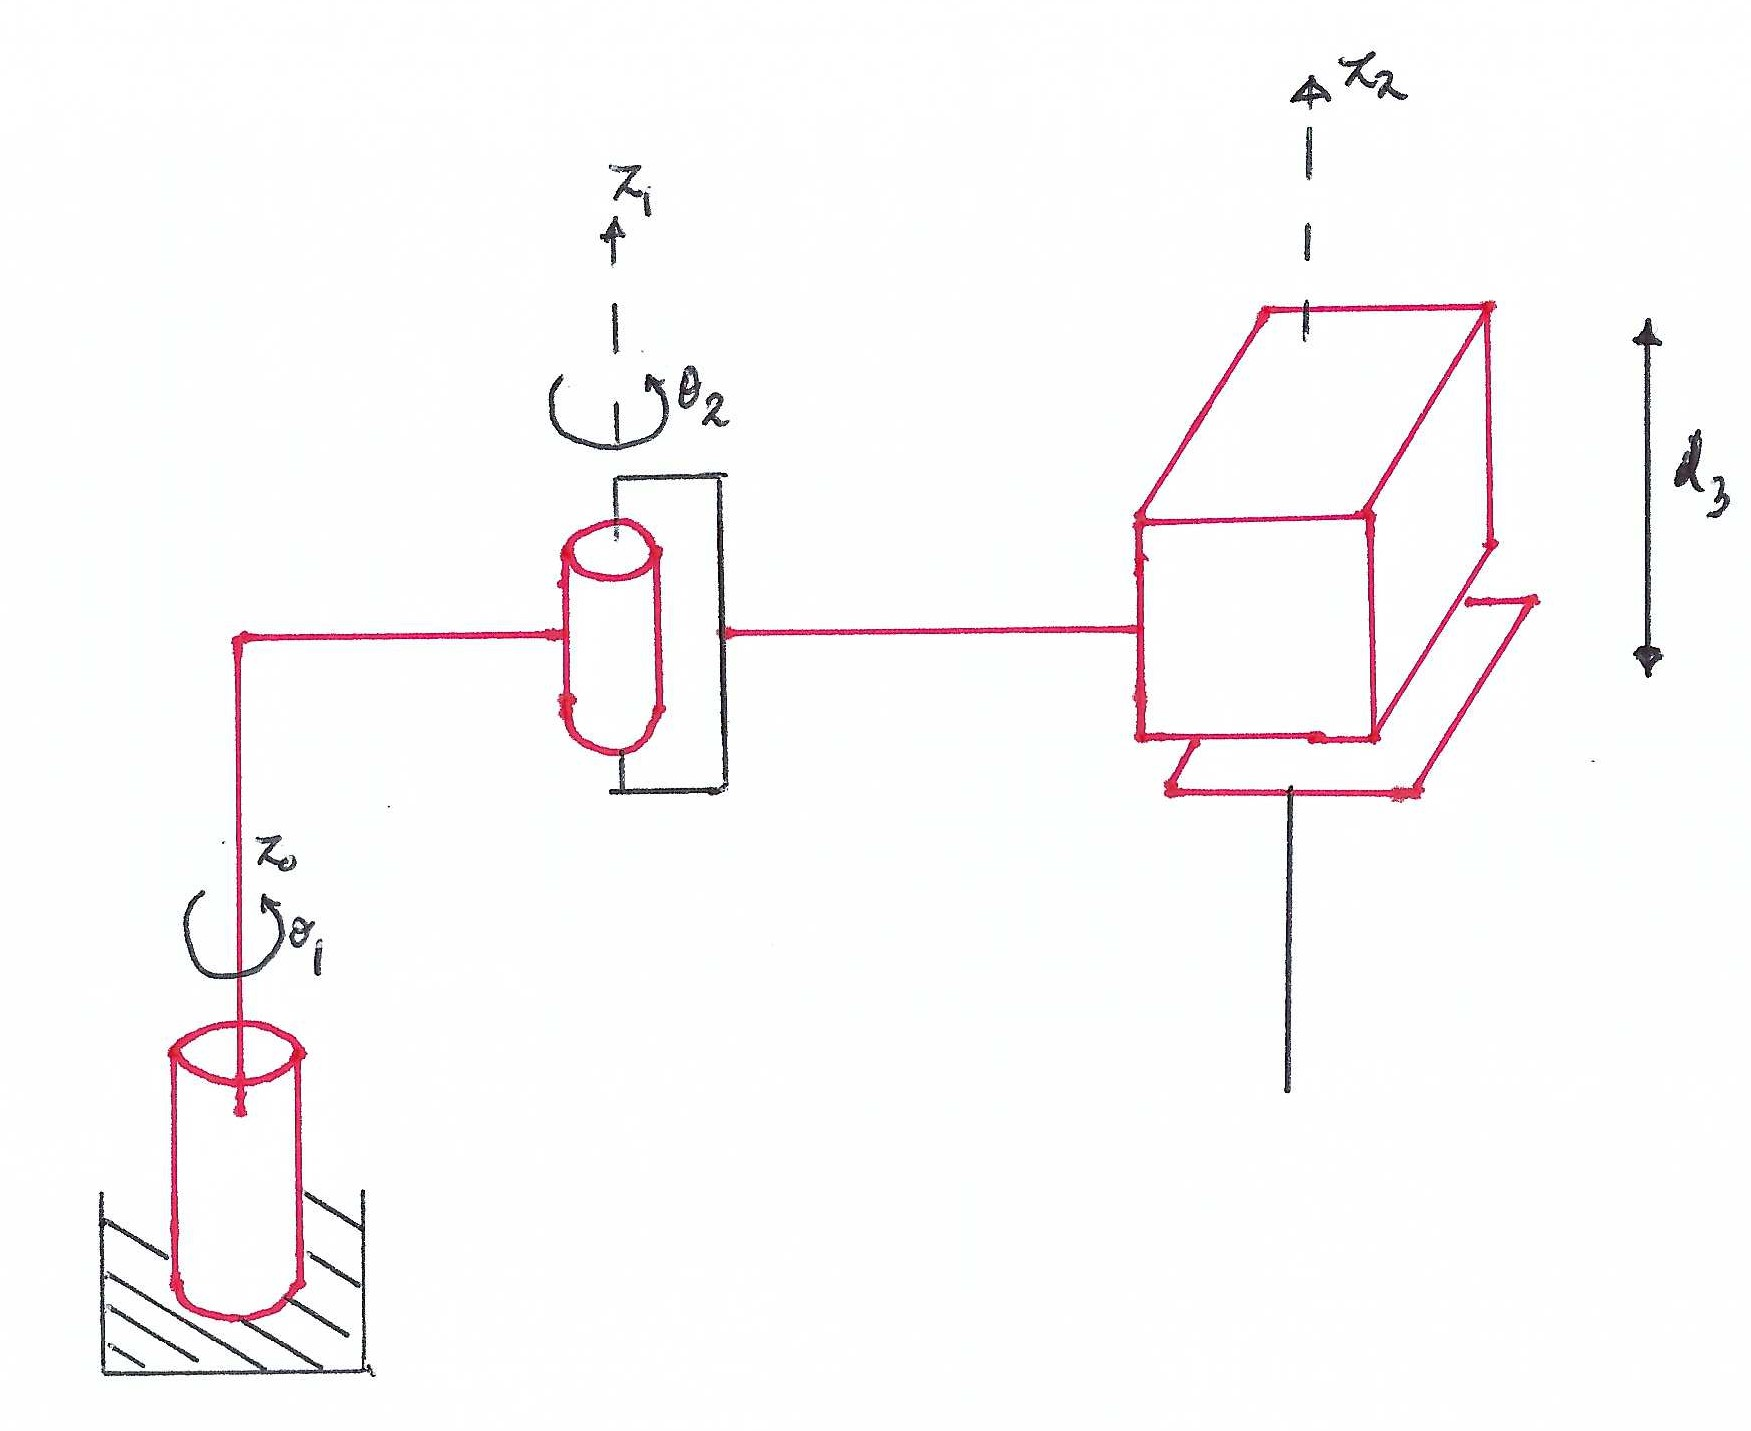
\includegraphics[width=\textwidth]{figures/scara_schematic.jpg}
			\footnotesize{Configuration of the SCARA Arm.}
		\end{column}
		%
		\begin{column}{.5\linewidth}
			\centering
			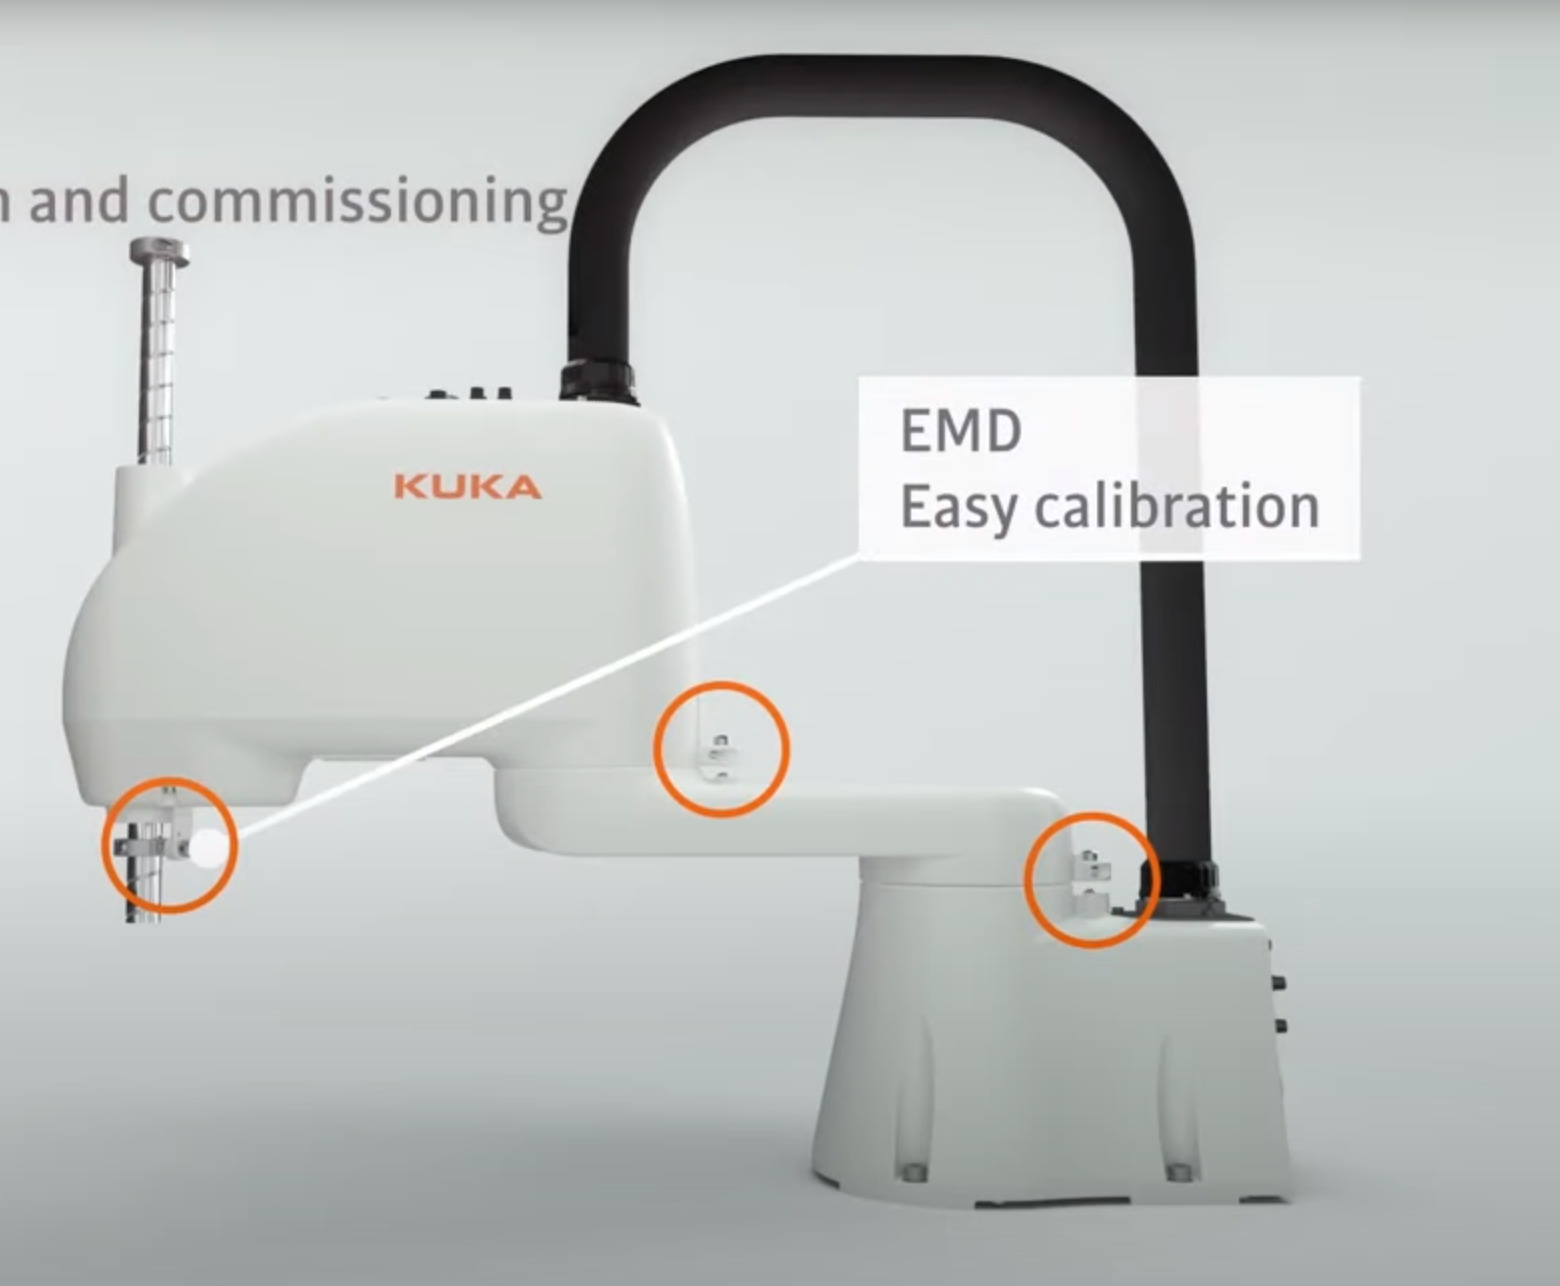
\includegraphics[width=\textwidth, rotate=360]{figures/Scara.jpg}
			\footnotesize{Courtesy of Fanuc America Inc.}
		\end{column}
	\end{columns}
\end{frame}
%
\begin{frame}
	\frametitle{Mobility of The SCARA Robot}
	%
	\begin{columns}[]
		%
		\begin{column}{.5\linewidth}
			\begin{block}{Mobility Analysis}
				Two rotary joints. One prismatic joint acting along the $z$ axis, and constrained along the $xy$ plane. 
			\end{block}
		\end{column}
	%
		\begin{column}{.5\linewidth}
			\begin{block}{Mobility Parameters}			
			Four rigid bodies (links). Three constraints.  Four freedoms. Therefore, $\mathfrak{M}=6(4-3-1)+4=4$
			\end{block}
		\end{column}
	\end{columns}
\end{frame}

\begin{frame}
	\frametitle{Mobility Analysis of The Universal Robot}
	%
	\begin{columns}[]
		%
		\begin{column}{.5\linewidth}
			\centering
			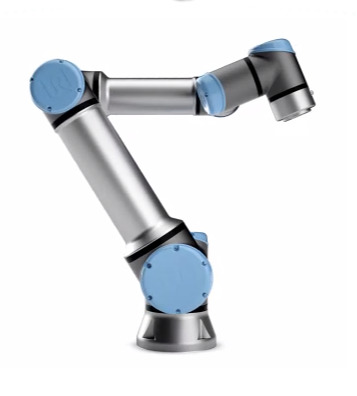
\includegraphics[width=\textwidth]{figures/ur16.jpg}
			\footnotesize{\copyright Universal Robots A/S, DK.}
		\end{column}
		%
		\begin{column}{.5\linewidth}
			\centering
			\begin{block}{The Revolute Arm}
				\footnotesize{Falls under so-called $RRR$ kinematic arrangements. Also called a \textcolor{blue}{revolute}, \textcolor{blue}{elbow}, or \textcolor{blue}{anthorpomorphic manipulator}.}
			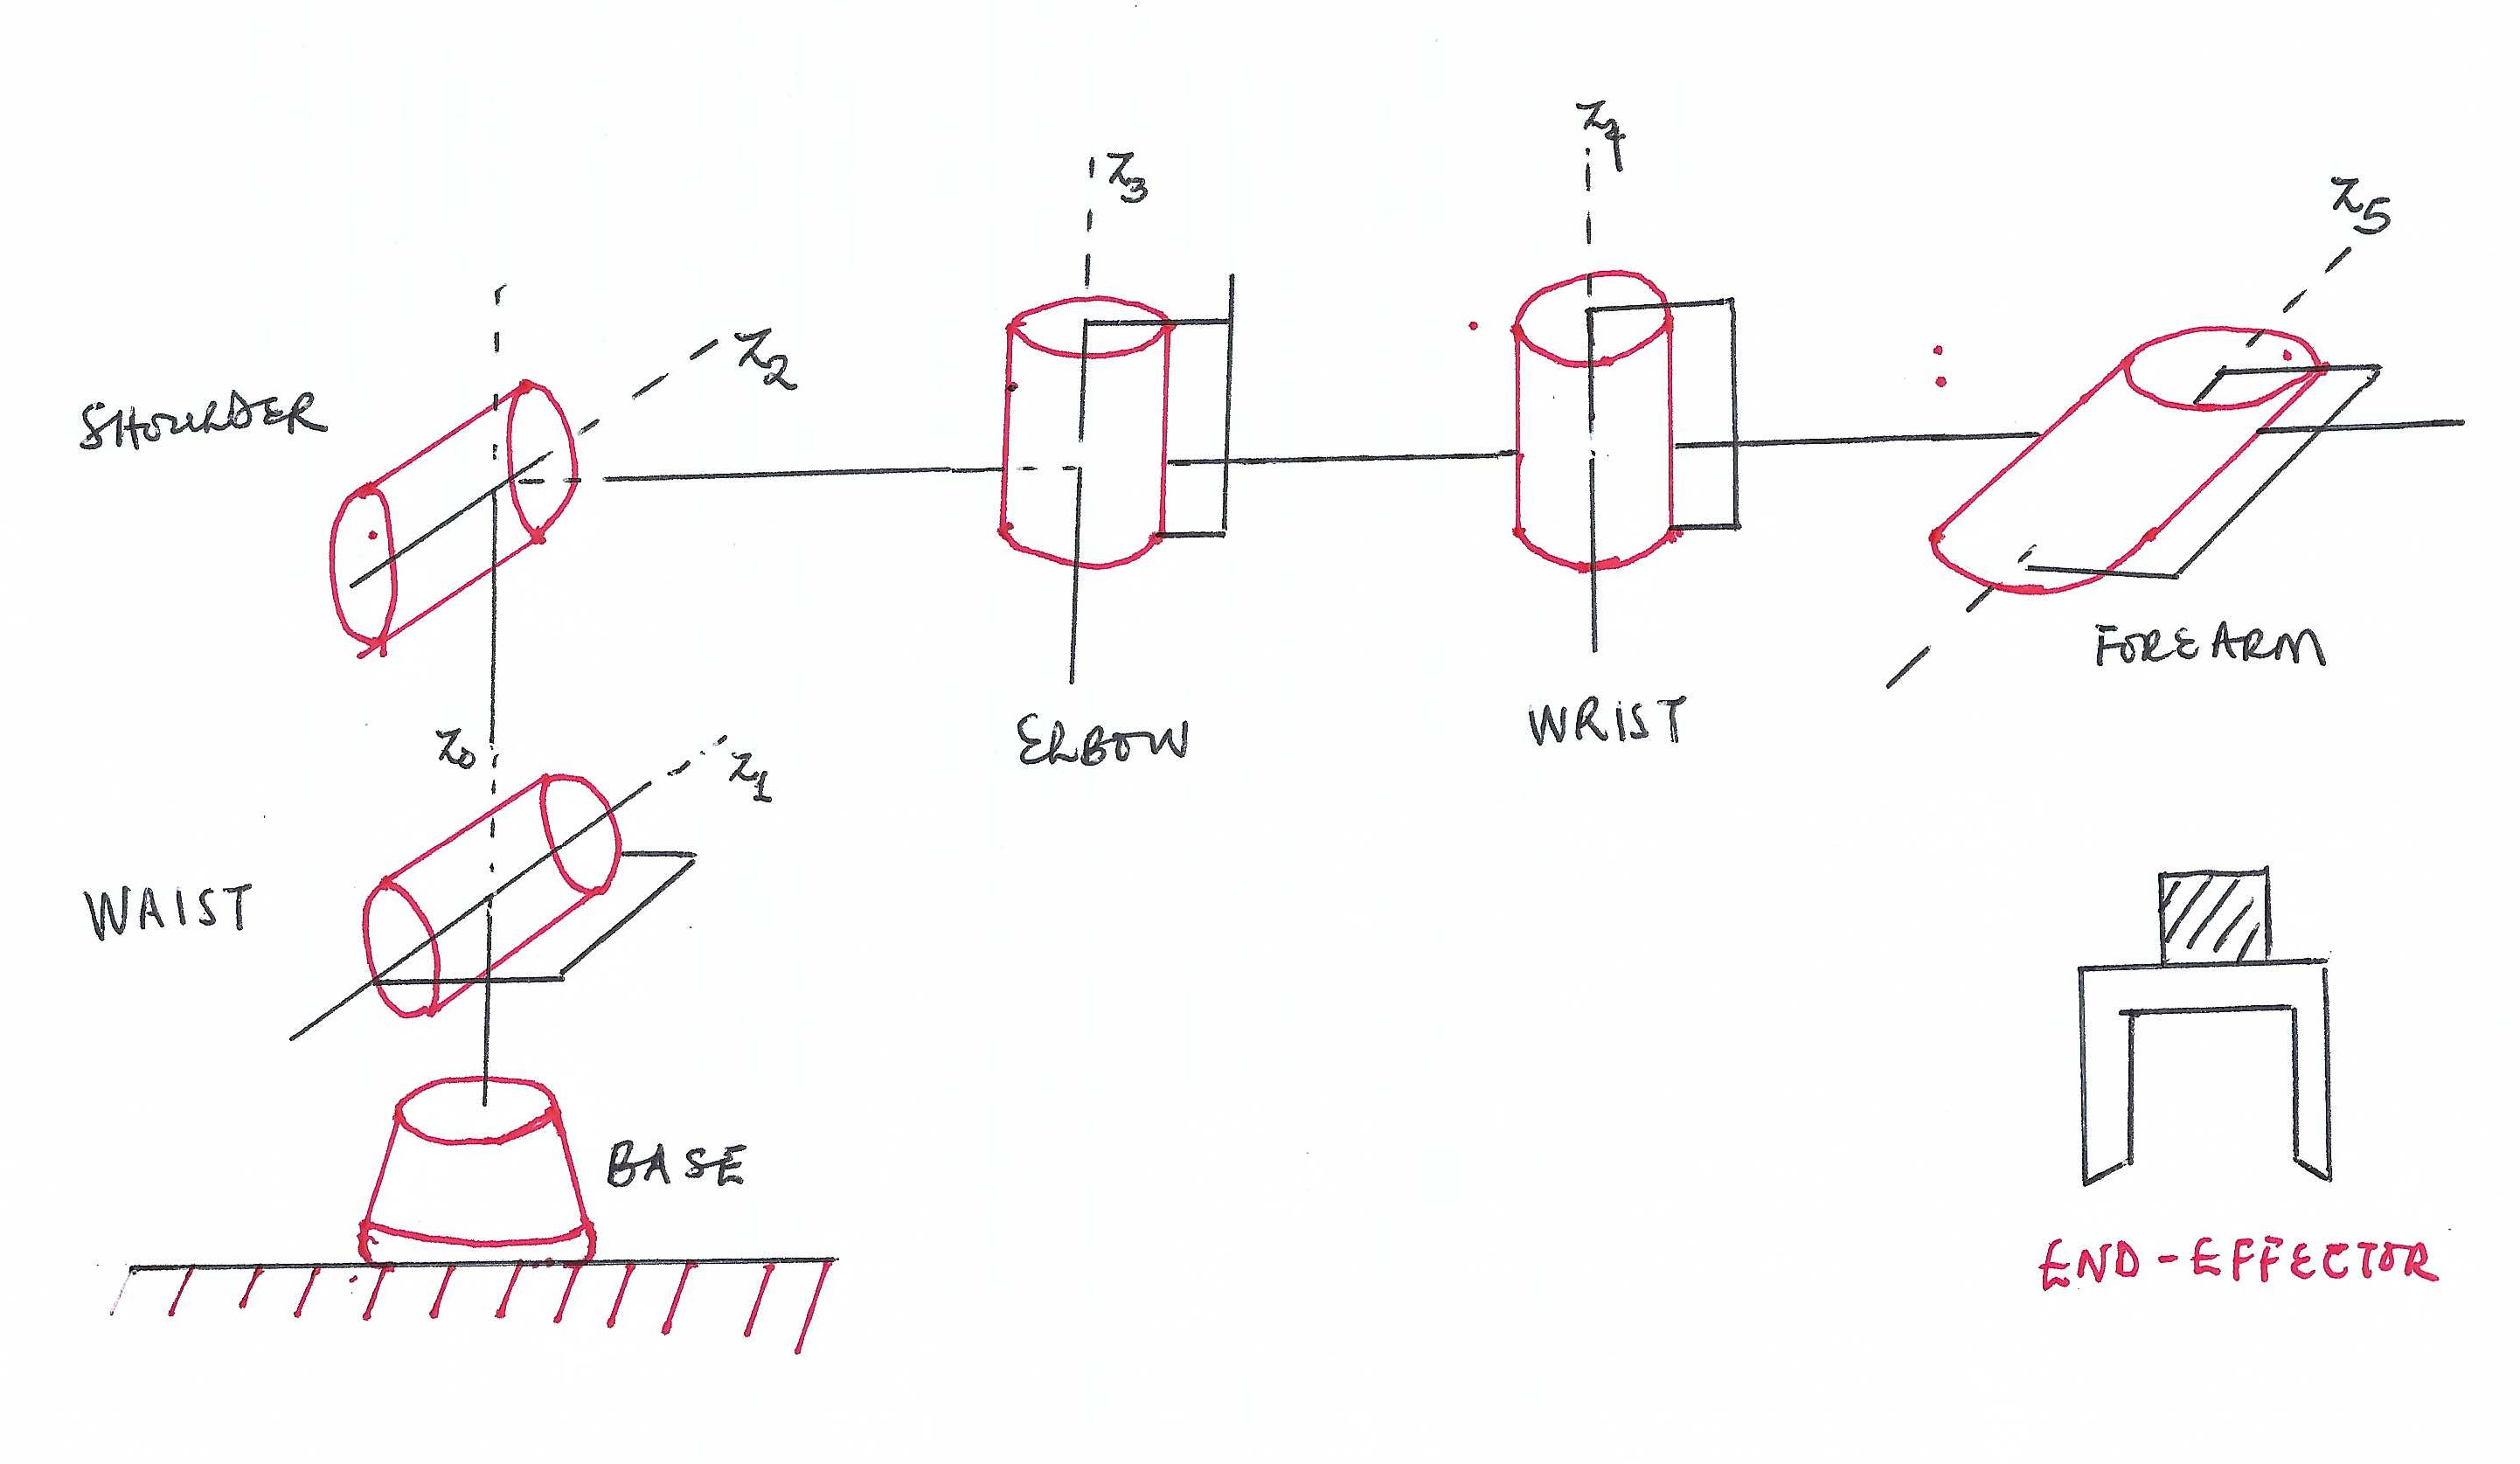
\includegraphics[width=\textwidth]{figures/ur_scheme.jpg}
			$n=6; \, k=6; \, f=5\times3:=18$ $\therefore \mathfrak{M}=6(n-k-1)+\sum f_i $ $\implies 6(6-1-5) + 18$ or $\mathfrak{M}=6$.
			\end{block}
		\end{column}
	\end{columns}
\end{frame}

\begin{frame}
	\frametitle{Mobility of The Stewart-Gough Platform}
	%	
	\centering 
	\begin{columns}
		\begin{column}{.4\linewidth}
			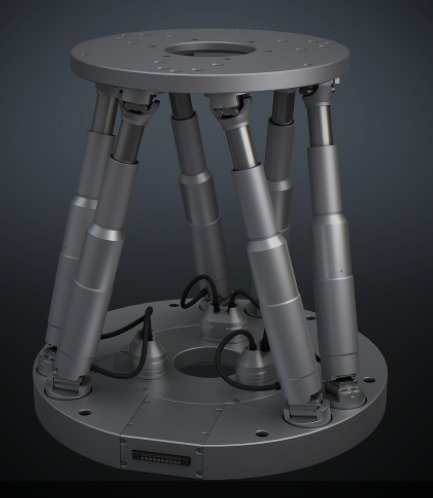
\includegraphics[width=\textwidth]{figures/stewart_spherical.jpg}
		\end{column}
		%\begin{columns}
		\begin{column}{.25\linewidth}
			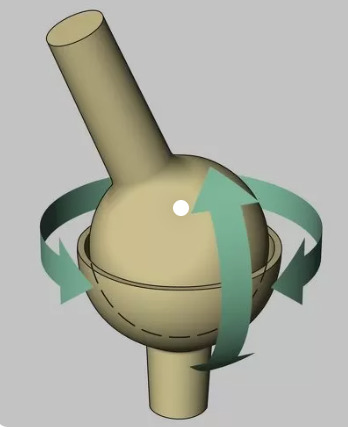
\includegraphics[width=\textwidth]{figures/spherical.jpg}
			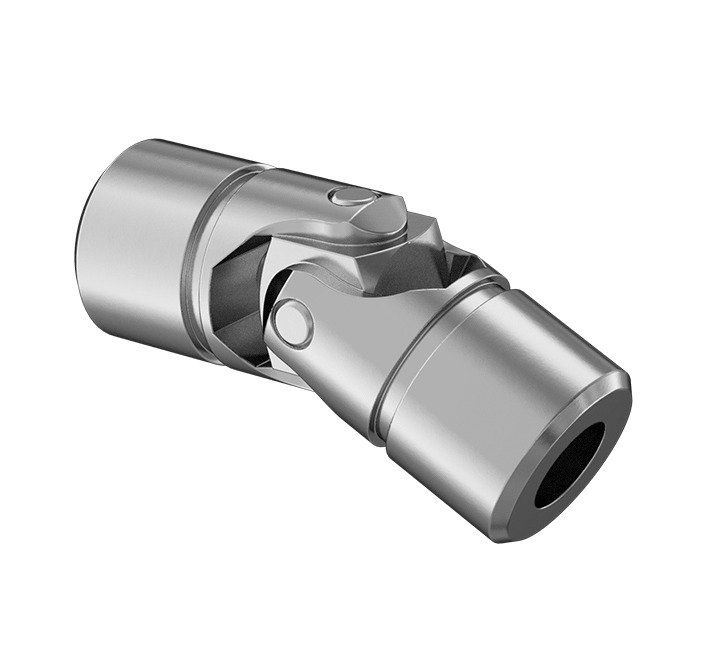
\includegraphics[width=\textwidth]{figures/ujoint.jpg}	
		\end{column}
		%\end{columns}
	\end{columns}	
\end{frame}

\begin{frame}
	\frametitle{Mobility of The Stewart-Gough Platform}
	%
	\begin{columns}[]
		%
		\begin{column}{.45\linewidth}
			\begin{block}{Unconstrained bodies, $n$}
				There are \textcolor{blue}{six universal joints} that connect \textcolor{blue}{the base platform} to the prismatic linear actuators. There are \textcolor{blue}{six spherical joints} that connect \textcolor{blue}{the top platform} to the top of the prismatic actuators. Altogether, there are $n=6+6+2$ or $14$ unconstrained \textcolor{red}{rigid links}.
			\end{block}
		\end{column}
		%
		\begin{column}{.55\linewidth}
			\begin{block}{Constraints, $k$}			
				Six \textcolor{blue}{u-joints}. Six \textcolor{blue}{spherical joints}.  Six \textcolor{blue}{prismatic joints}. Altogether, there are $f=6+6+6:=18$ \textcolor{blue}{constraints}.
			\end{block}
			\begin{block}{Freedoms, $f$}			
				Each \textcolor{blue}{u-joints has two freedoms}. Each \textcolor{blue}{spherical joint has three (rotary) freedoms}.  Each \textcolor{blue}{prismatic joint has one freedom}. Altogether, there are $f=6\times2+6\times3+6\times1:=36$ \textcolor{blue}{freedoms}.
			\end{block}
		
		\end{column}
	\end{columns}
\end{frame}
